\chapter{The proposed approach}
In the thesis we propose a new and innovative system for the white blood cells segmentation and counting based on the Vector Field Convolution.

\bigskip
In the diagram \ref{fig:diag} the scheme of the proposed system is showed. In the first phase we acquire the image containing the cells. In the second step the mean-shift method is applied in order to obtain a better image for the segmentation. In the third step we apply the VFC method in order to obtain the intensity image. The fourth step transform the intensity image in a grade image where each pixel has a specific direction. The fifth and the sixth steps are parallels. In the fifth step we calculate the external energy and the  distance transform on the grade image. In the sixth step the median filter is applied on the results of the fifth step. The seventh step shows the overlay between the two results of the sixth step in order to detect only the leukocytes. The eighth step applies the skeleton method in order to do an initial segmentation. The ninth step applies the region merging function to segment and finally count the cells in the image. 
\begin{figure}
	\begin{center}
		\centering
		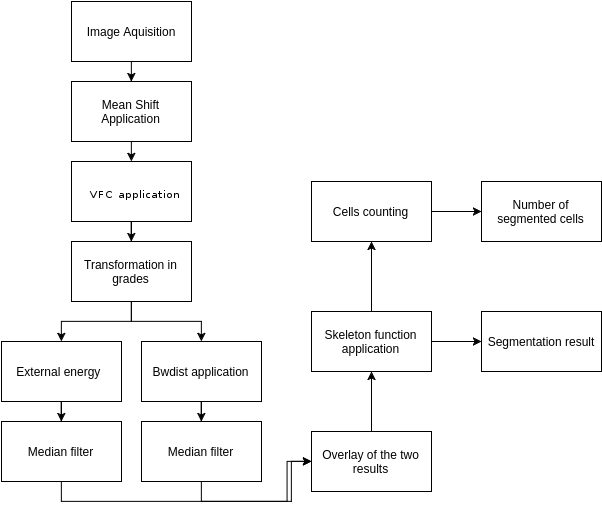
\includegraphics[scale=0.5]{img/diag.png}
		\caption{Method diagram representation}
		\label{fig:diag}
	\end{center}
\end{figure}

\bigskip

As we can see in literature, the main approach used to resolve the overlap problem is using the watershed transform \cite{water}. In figure (\ref{fig:overlap}) there is an example of the watershed transform. Taken in input the image of the two overlapped circles, we calculate the distance transform, or in other words we calculate the Euclidean distance transform of the binary image BW. For each pixel in BW, the distance transform assigns a number that is the distance between that pixel and the nearest non-zero pixel of BW (\ref{fig:overlaptransf}). Giving the distance transform result to the watershed algorithm we obtain a division between circles because the watershed transform finds "catchment basins" or "watershed ridge lines" in an image by treating it as a surface where light pixels represent high elevations and dark pixels represent low elevations (\ref{fig:overlapwater}).
\begin{figure}[htbp]
    \centering
    \begin{subfigure}[b]{0.5\textwidth}
        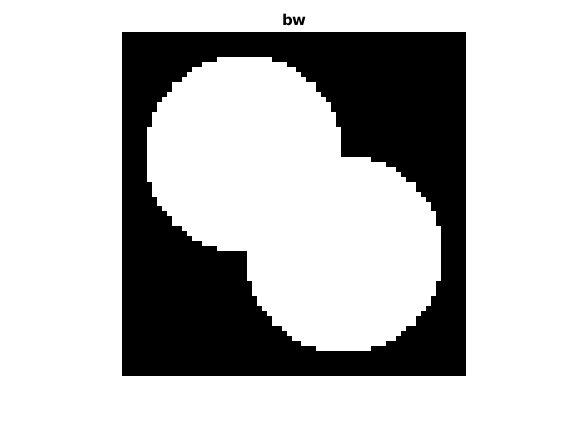
\includegraphics[width=\textwidth]{img/circlesEx.png}
        \caption{ }
        \label{fig:overlap}
    \end{subfigure}
     \quad
      %(or a blank line to force the subfigure onto a new line)
    \begin{subfigure}[b]{0.5\textwidth}
        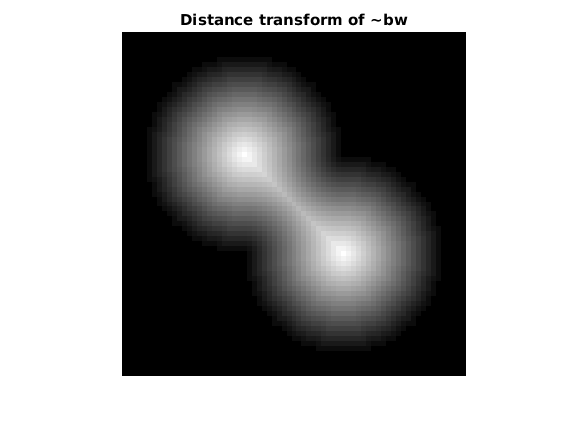
\includegraphics[width=\textwidth]{img/distancerTransform.png}
        \caption{ }
        \label{fig:overlaptransf}
    \end{subfigure}
    \quad
    \begin{subfigure}[b]{0.5\textwidth}
        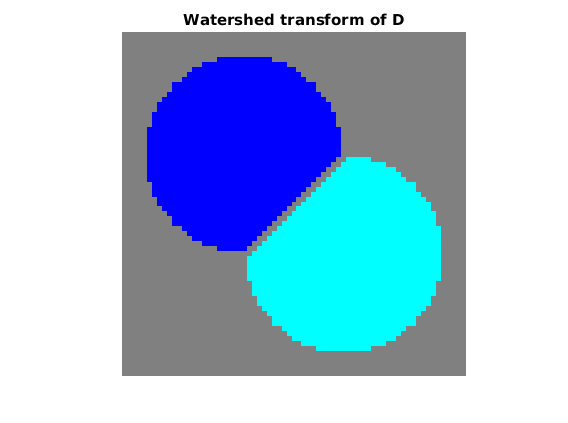
\includegraphics[width=\textwidth]{img/watershedEx.png}
        \caption{ }
        \label{fig:overlapwater}
    \end{subfigure}
    \caption{(a) Example of two circle in overlap, (b) Distance transform, (c) Watershed result}\label{fig:stepswater}
\end{figure}
This is an ideal case to analyse. But when we work with the overlapping between cells the result of the division by watershed transform is not optimal like the example \ref{fig:stepswater}. Probably the cause derives from the low definition of the figures and especially the shape of the cells. Here there is an example of what happens when we try to divide three cells in overlap (\ref{fig:exOnImage7}).
\begin{figure}
	\centering
	\begin{subfigure}[b]{0.5\textwidth}
        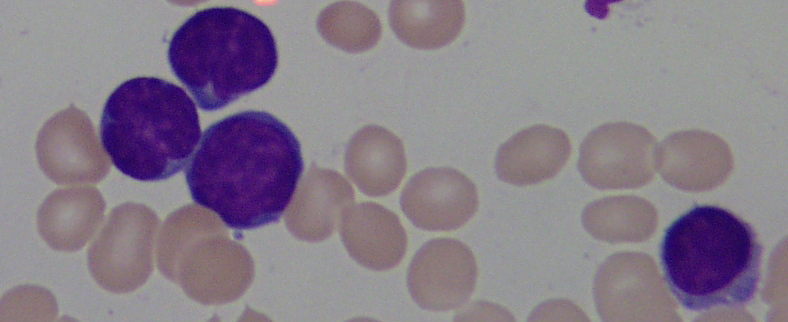
\includegraphics[width=\textwidth]{img/Im007_1_crop.png}
        \caption{ }
        \label{fig:origimage}
    \end{subfigure}
    \begin{subfigure}[b]{0.5\textwidth}
		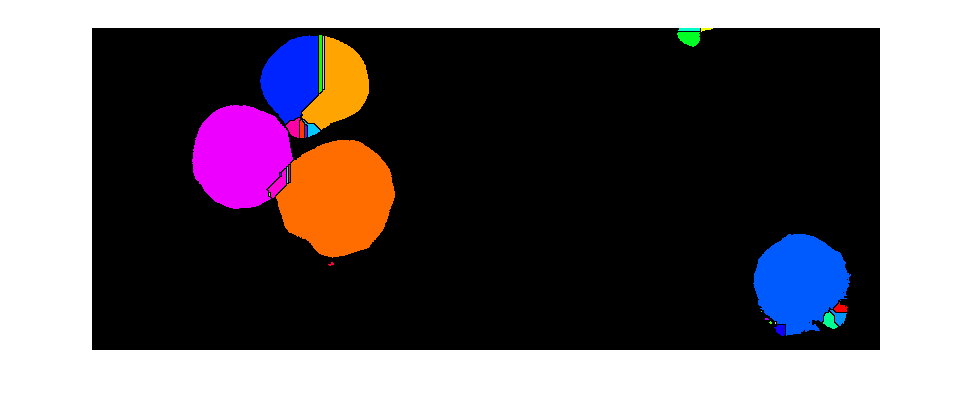
\includegraphics[width=\textwidth]{img/waterTrRes.png}
		\caption{ }
		\label{fig:watershedoncells}
	\end{subfigure}
	\caption{(a) Original leukocytes image, (b) Watershed transform applied to three cells in overlap}
	\label{fig:exOnImage7}
\end{figure}
As it is possible to see, this method produces a no-realistic separation of the cells. For this reason we study a different method that in automatic way produces a realistic division of the cells. Starting from the resulting image after the application of the mean shift algorithm, we based our implementation using principally the output of the VFC field, the image relative to the External energy of the image to describe the edges, the median filter, the skeleton method and the region-merging function.

\bigskip
The proposed system has been tested on images belonging to a public dataset, the ALL-IDB blood cell dataset \cite{idbpaper}.

\section{ALL-IDB blood cell dataset}
The images of the dataset have been captured with an optical laboratory microscope coupled with
a Canon PowerShot G5 camera. All images are in JPG format with 24-bit colour depth. The first 33
have $1712*1368$ resolution, the remaining have $2592*1944$ resolution. The images are taken with
different magnifications of the microscope ranging from 300 to 500 which brings the colour
differences that we managed grouping the images with same brightness characteristics together. The
ALL-IDB database has two distinct folders (ALL-IDB1 and ALL-IDB2).

\bigskip

The table \ref{tableidb} shows a little description about the images.
\begin{table}
\centering
\begin{tabular}{|c|c|c|}
\hline 
Characteristic & ALL-IDB1 & ALL-IDB2 \\ 
\hline 
Images & 109 & 260 \\ 
\hline 
Max resolution & 2592x1944 & 257x257 \\ 
\hline 
Elements & 39000 & 260 \\ 
\hline 
Candidate Lymphoblasts & 510 & 130 \\ 
\hline 
\end{tabular} 
\caption{Characteristics of the dataset. Images acquisition has been performed with a Canon PowerShot G5. Magnification of microscope goes from 300 to 500. The image format of the ALL- IDB1 folder images is JPG, ALL-IDB2 images have TIF format. The colour is 24 bit depth.}
\label{tableidb}
\end{table}
The IDB1 set can be used for testing segmentation capability of algorithms. This dataset is composed of 108 images collected during September, 2005. It contains about 39000 blood elements, where the lymphocytes have been labelled by expert oncologists.\cite{website:IDB}
The IDB2 set has been designed for testing the performances of classification systems. The ALL-IDB2 version 1.0 is a collection of cropped area of interest of normal and blast cells that belongs to the ALL-IDB1 dataset. ALL-IDB2 images have similar gray level properties to the images of the ALL-IDB1, except the image dimensions.\cite{website:IDB}
For our work we considerchangesed only normal type of leukocytes and we focused principally on the images where is present an overlap between the white blood cells.

\section{Mean shift application}
In order to resolve the illumination problems and to obtain a good visualization of the Wright-Giemsa stain cells we use the mean shift function. To obtain an acceptable result it should be necessary an image preprocessing, but using the bandwith parameters and the threshold parameter of the mean shift function we can obtain the same result. For our work we used $h_{s}$ (bandwith of the spatial kernel) = 4, $h_{r}$ (colour bandwith) = 4 and the threshold $th$ = 0.25. The result obtained by changing these parameters is not so significant in order to obtain a good final result, then is preferable use an image with a little bit definition but obtained in a very short time (2 seconds for cropped images and 40 seconds for the entire images). To understand what are the differences in the image when we apply the mean shift procedure, is appropriate do a comparison between the images before and after the application of the method (\ref{fig:mean}). The resulting image is very helpful to calculate the edge map that will give as parameter to the VFC function.
\begin{figure}
	\centering
	\begin{subfigure}[b]{1\textwidth}
        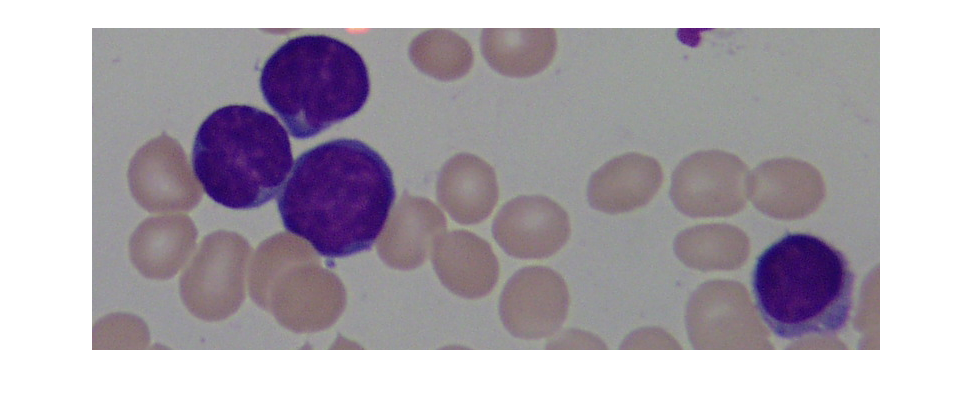
\includegraphics[width=\textwidth]{img/final/menorig.png}
        \caption{ }
        \label{fig:meanorig}
    \end{subfigure}
    \begin{subfigure}[b]{1\textwidth}
		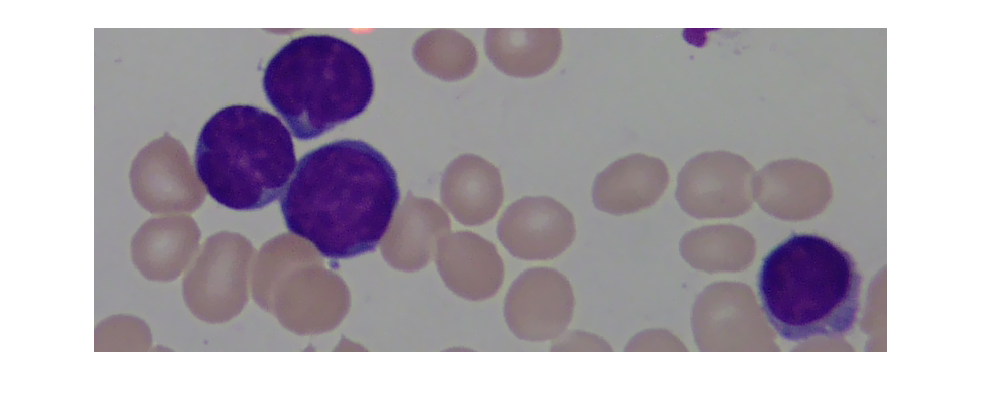
\includegraphics[width=\textwidth]{img/final/meanshift.png}
		\caption{ }
		\label{fig:meanshift}
	\end{subfigure}
	\begin{subfigure}[b]{1\textwidth}
		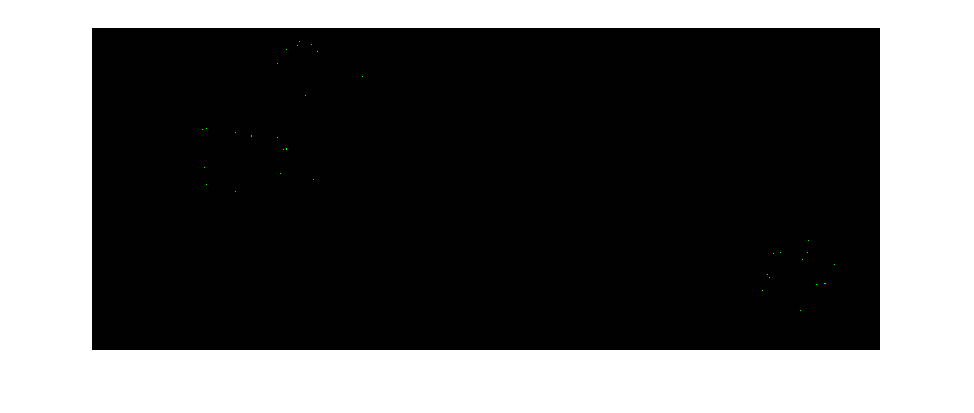
\includegraphics[width=\textwidth]{img/final/meanshiftdifferenceimage.png}
		\caption{ }
		\label{fig:meandifference}
	\end{subfigure}
	\caption{(a) Original image, (b) Mean-shift result, (c) Difference between mean-shift image and original image}
	\label{fig:mean}
\end{figure}

\section{The VFC result}
The VFC uses the two components of the external force ${u} _{vfc} ( x,y ) , {v} _{vfc} (x,y)$ to describe the field of the image and its magnitude. Our purpose is find an image using these two components that describes all the leukocytes edges taking an accurate look on the edges in overlap and in clump. The first step then is extract the right component and the left component by the VFC field.
\begin{equation}
{u} _{vfc}=ExtF(x)/\sqrt{ExtF(x)^{2} + ExtF(y)^{2}}
\end{equation}
\begin{equation}
{v} _{vfc}=ExtF(y)/\sqrt{ExtF(x)^{2} + ExtF(y)^{2}}
\end{equation}
ExtF is the External force of the field. Now we have only an intensity image, but to understand how the field moves in the space we have to transform these two component $ u$ and $ v $ in grades. We want to understand the direction of every pixel in the figure especially the pixels that describe edges of cells. It is possible to convert the two components in degrees using the $atan2d$ function \ref{fig:angle}.
\begin{figure}
	\begin{center}
		\centering
		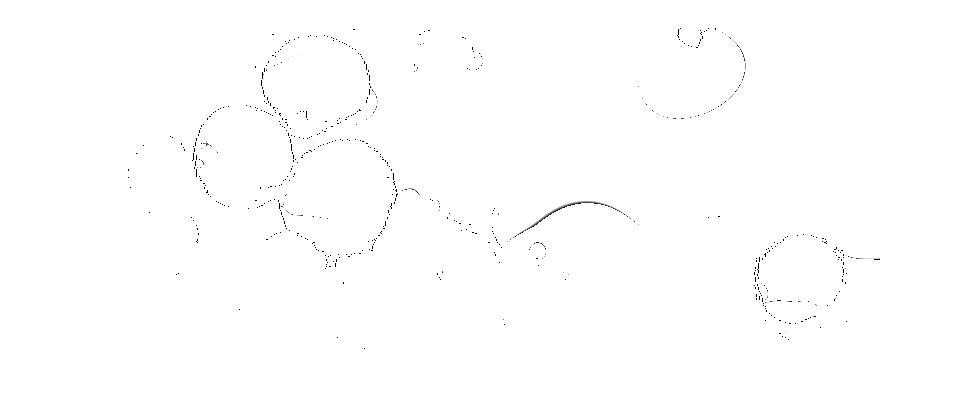
\includegraphics[scale=0.5]{img/angle.png}
		\caption{Degrees image}
		\label{fig:angle}
	\end{center}
\end{figure}
In order to delete all the uniform part of the figure and put in exalt the edges we use a mediand filter using the function $ordfilt2$ searching the 18th element of the $5 * 5$ mask (\ref{fig:Pmedangle}).
\begin{figure}
	\begin{center}
		\centering
		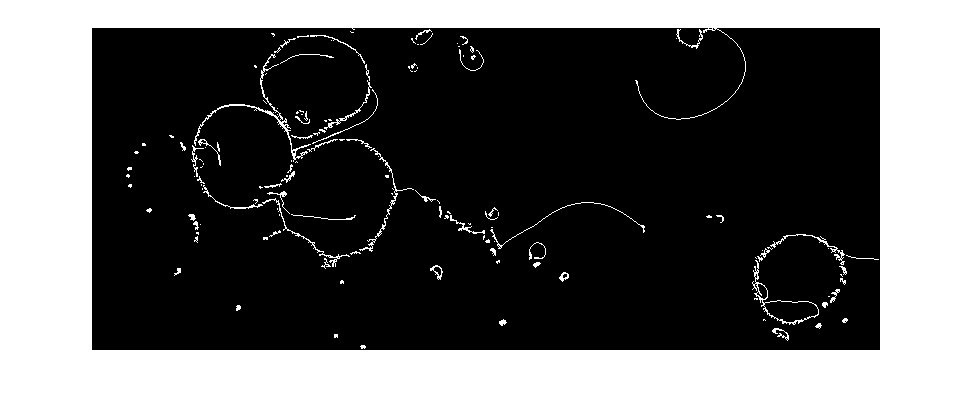
\includegraphics[scale=0.5]{img/PmedAngle.png}
		\caption{Median filter on degrees image}
		\label{fig:Pmedangle}
	\end{center}
\end{figure}
\section{External Energy}
As it is possible to see in the result \ref{fig:angle}, there are a lot of points that are artefacts created by the field. For these reason we used the $bwdist$ function to assign a number that it is the distance between each pixel and the nearest no-zero pixel of the image. This trick is very useful because it reduces the entropy of the image, focusing only on the shape of the leukocytes (\ref{fig:bwdistangle}).
\begin{figure}
	\begin{center}
		\centering
		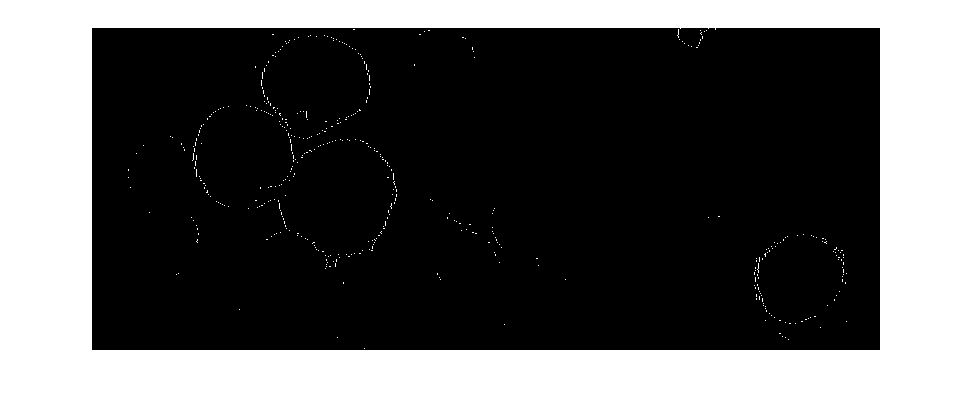
\includegraphics[scale=0.5]{img/bwdistAngle.png}
		\caption{bwdist applied on degrees image}
		\label{fig:bwdistangle}
	\end{center}
\end{figure}
But we have still the same problem. In the image there are trace of the red blood cells, then we had to find a method to isolate only the leukocytes. We started using the external energy of the image. For an image $I(x,y)$ all the lines, edges and terminal points the general formulation of the Energy of the image is
\begin{equation}
 E_{image}=w_{line}E_{line} + w_{edge}E_{edge} + w_{term}E_{term}
\end{equation}
where $w_{line}, w_{edge}, w_{term}$ are weights of the features.

\subsection{Line functional}
The line functional or in other terms the intensity of the image is in a nutshell the attracted value of the dark lines to the light line. Is possible choose this attraction putting a positive or negative sign before the force that this attraction has to be.
\begin{equation}
	E_{{line}}=filter(I(x,y))
\end{equation}

\subsection{Edge functional}
The edge functional bases its work on the image gradient.
\begin{equation}
E_{{edge}}=-\left|\nabla I(x,y)\right\vert ^{2}
\end{equation}
It's very useful because when we try to analyse the feature of the image, we work with maxims and minims. With this formula we can avoid the local minima that are not object of interest. The energy functional using scale space continuation is
\begin{equation}
E_{edge}=-\left|G_{\sigma }*\nabla ^{2}I\right\vert ^{2}
\end{equation}
where $ G_{\sigma } $ is a Gaussian with standard deviation $ \sigma $.

\subsection{Termination functional}
The curvature of the lines in a image is utilized to detect corners and terminations. Put 
\begin{equation}
C(x,y)=G_{{\sigma }}*I(x,y)
\end{equation}
with a gradient angle
\begin{equation}
\theta =\arctan {\Bigg (}{\frac  {C_{y}}{C_{x}}}{\Bigg )},
\end{equation}
unit vectors that move along the gradient direction 
\begin{equation}
{\mathbf  n}=(\cos \theta ,\sin \theta )
\end{equation}
and unit vectors perpendicular to the gradient direction
\begin{equation}
{\mathbf  n}_{{\perp }}=(-\sin \theta ,\cos \theta ).
\end{equation}
With these 4 equations we can describe the termination functional of energy as follow
\begin{equation}
E_{{term}}={\partial \theta  \over \partial n_{{\perp }}}={\partial ^{2}C/\partial ^{2}n_{{\perp }} \over \partial C/\partial n}={{C_{{yy}}C_{x}^{2}-2C_{{xy}}C_{x}C_{y}+C_{{xx}}C_{y}^{2}} \over (C_{x}^{2}+C_{y}^{2})^{{3/2}}}
\end{equation}

\subsection{External energy result}
Now we have only to specify the value of each parameter as explained above.
To obtain the desired outcome we did some empirical experiments, obtaining the best result with $ Wedge=8, Wline=-8 $ and $ Wterm=0$. This result (\ref{fig:Eextforce}) permit us to extract only the leukocytes part of the image using some analysis image exploit (\ref{fig:onlyleu}).

\begin{figure}
	\begin{center}
		\centering
		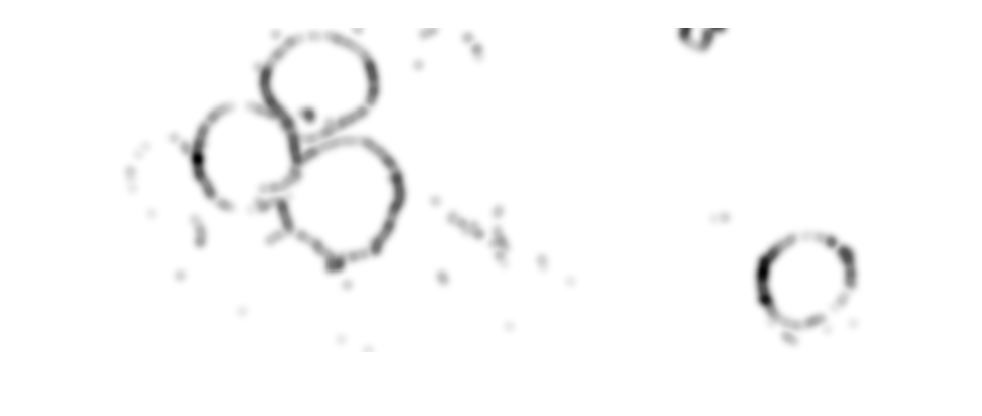
\includegraphics[scale=0.5]{img/Eext.png}
		\caption{External energy result}
		\label{fig:Eextforce}
	\end{center}
\end{figure}
\begin{figure}
	\begin{center}
		\centering
		
\includegraphics[scale=0.5]{img/onlyleuco.png}
		\caption{External energy image of leukocytes without red blood cells}
		\label{fig:onlyleu}
	\end{center}
\end{figure}
\bigskip

In order to delete all the uniform part of the figure and put in exalt the edges we use a mediand filter using the function $ordfilt2$ searching the 18th element of the $5 * 5$ mask \ref{fig:Pmedonlyleu}.

\begin{figure}
	\begin{center}
		\centering
		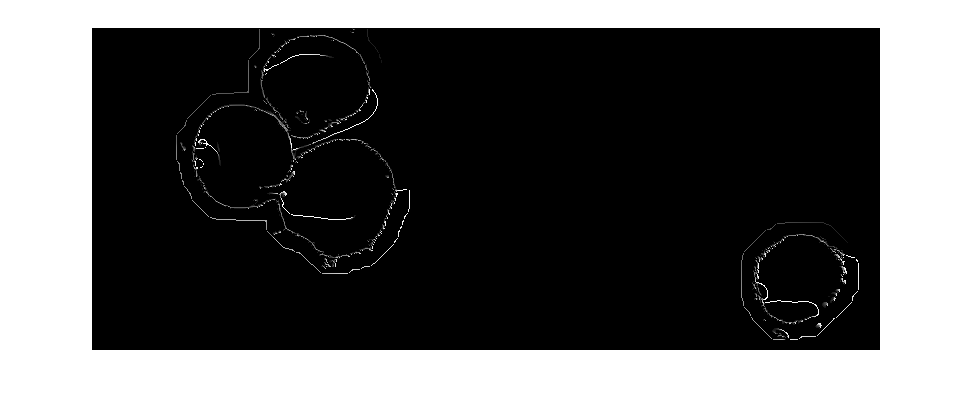
\includegraphics[scale=0.5]{img/Pmedonlyleuko.png}
		\caption{edges and region}
		\label{fig:Pmedonlyleu}
	\end{center}
\end{figure}
\section{Combination of two results: the division method}
The two obtained results seem in no-correlation, but the skill of this segmentation lives in this passage. Using the overlay function we search all the points in overlay between the median filter application on the degrees image and the edges region, using the red color to isolate the leukocytes region \ref{fig:over}.
\begin{figure}
	\begin{center}
		\centering
		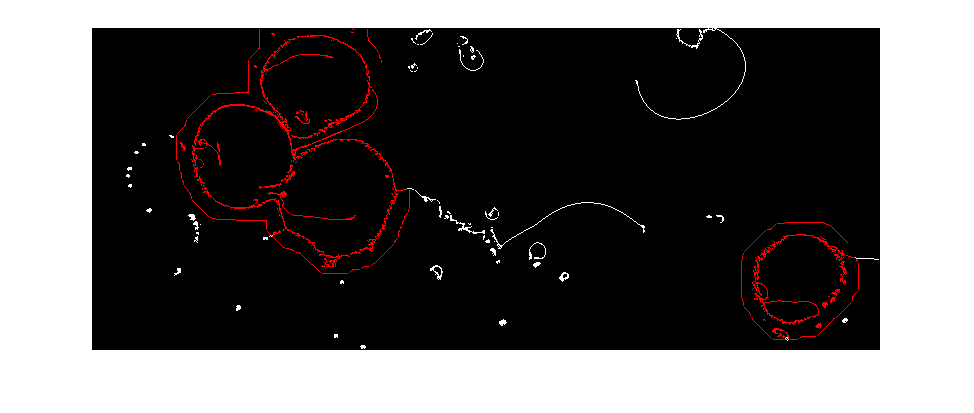
\includegraphics[scale=0.5]{img/overlay.png}
		\caption{overlay of figures \ref{fig:Pmedangle} and \ref{fig:Pmedonlyleu}}
		\label{fig:over}
	\end{center}
\end{figure}
We choose to use the red color, because by isolating only the red component of the image we can obtain an image that contains only the leukocytes regions. The result of this task is visible in the image \ref{fig:leukoover} 
\begin{figure}
	\begin{center}
		\centering
		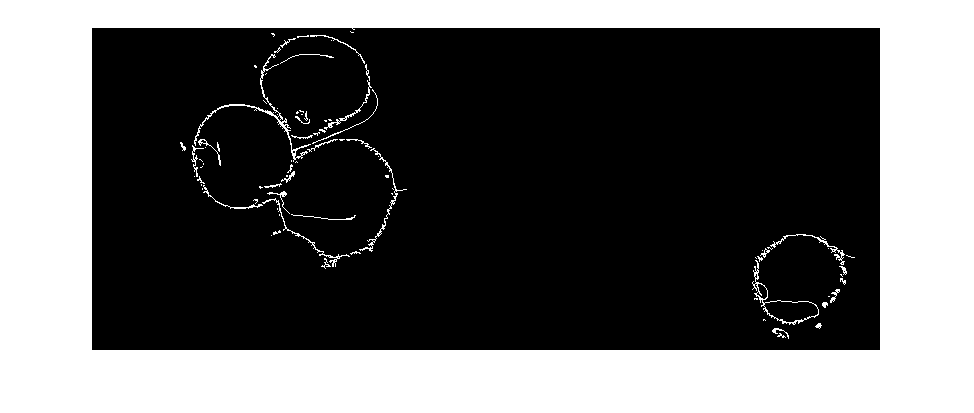
\includegraphics[scale=0.5]{img/overLeuko.png}
		\caption{only leukocytes edges}
		\label{fig:leukoover}
	\end{center}
\end{figure}

\section{Segmentation with the skeleton function}
Starting from the image containing only the edges we have to connect every single white point to the nearest in order to get a connected boundary of the objects. To do this task we use the function $imdilate$ to dilate all the white dots with a diamond structural element with the size of 6 pixels. After this step we apply the closing of the opening with two disk respectively of the size 3 and 4 pixels. Now we can apply the skeleton function or the thinning of the edges. To do this passage we use the Matlab function $bwmorph$ that it's not the best function to do this but is the faster one. We try another skeleton external function written by N. Howe that is very interesting because has a precision to compute the skeleton of the image that is very impressive, but because the Pc latency we can't use the last one function. After the skeleton application we obtain an image that contains some spurious branches (\ref{fig:skel}). 

\bigskip

To solve this problem is possible to use the Matlab function $bwmorph$ to prune the spurious branches, but in this case the function doesn’t work very well. For this reason we implement an alternative code to resolve the problem. Our code is like a parser that for each point sees if it is a part of a closed circle or not. If it's not a part of a loop the code deletes this point. In a nutshell we save only the point that stay in a 'road' with the starting point and the end point coincident. Below you can read a snippet of pruning code.
\begin{figure}
	\begin{center}
		\centering
		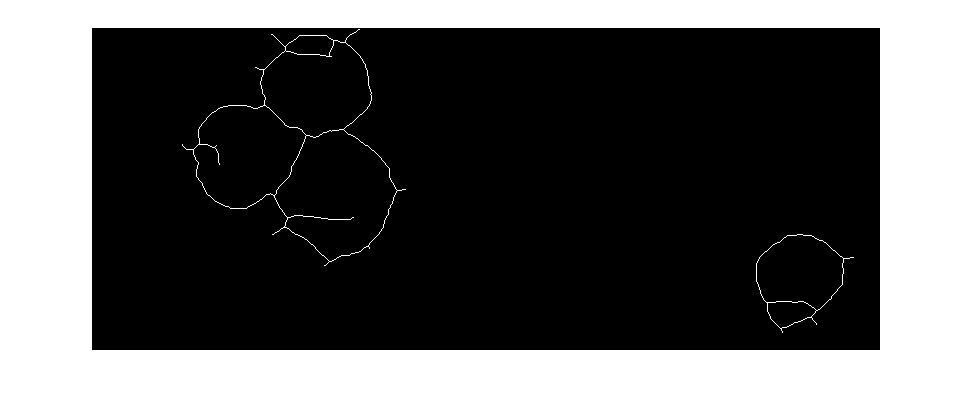
\includegraphics[scale=0.5]{img/skel.png}
		\caption{skeleton of leukocytes with irregular branches}
		\label{fig:skel}
	\end{center}
\end{figure}

\begin{minipage}{\linewidth}
\begin{scriptsize}
	\begin{lstlisting} [frame=single]
B = branchpoints;
E = endpoints;
[y,x] = Image;
Dmask = false(size(skel));
	for k = 1:numel(x)
    	D = bwdistgeodesic(skel,x(k),y(k));
    	distanceToBranchPt = min(D(B));
    	Dmask(D < distanceToBranchPt) =true;
	end
skelD = skel - Dmask;
	\end{lstlisting}
\end{scriptsize}
\end{minipage}
The result that we obtain from the skeleton application is a summary work, indeed we obtain an over-segmentation as is viewable from the image \ref{fig:skelfin}.
\begin{figure}
	\begin{center}
		\centering
		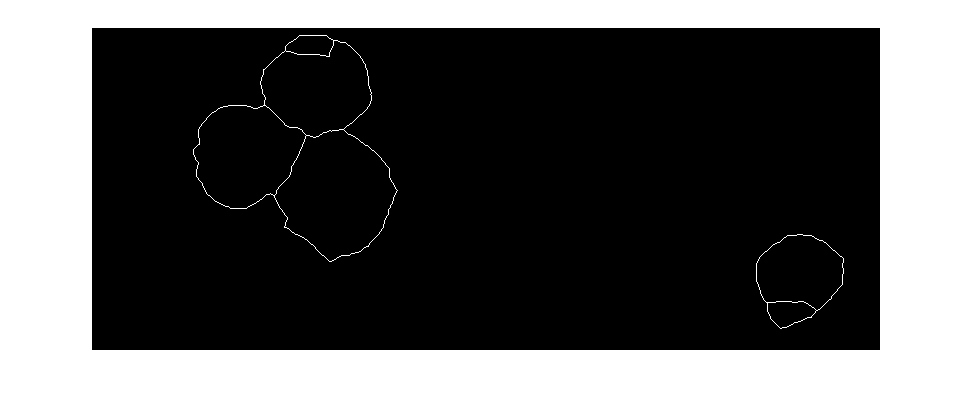
\includegraphics[scale=0.5]{img/skelfin.png}
		\caption{skeleton of leukocytes with no spurious branches}
		\label{fig:skelfin}
	\end{center}
\end{figure}
This over-segmentation isn't good for the correct visualization of leukocytes, but gives us a starting point to improve the solution and to obtain a better result.
Then we try to combine the various result to obtain a segmentation that was similar to the original image. First of all we close all the holes that are inside the image, to obtain a sort of black and white mask. Another fundamental step is summing the skeleton image with the mask. Doing this step we can separate the foreground by the background. Now we can use for the last time the map of edges that we used to calculate the VFC field. Doing an opening with a disk structural element with radius of 6 pixels and summing it with the image of leukocytes in foreground  we can can extract all connected components using the function $bwareafilt$. We do this because this function extracts all connected components (objects) from a binary image where the area is in range, producing the first segmented image of the leukocytes (\ref{fig:bwarea}).
\begin{figure}
	\begin{center}
		\centering
		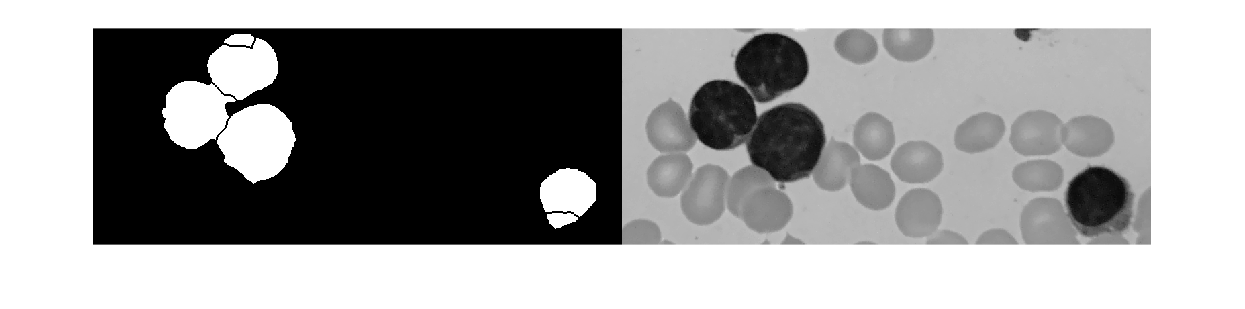
\includegraphics[scale=0.3]{img/segmentation.png}
		\caption{final leukocytes segmentation }
		\label{fig:bwarea}
	\end{center}
\end{figure}

\section{Cells counting}
\subsection{Detection and deletion of small over-segmentation areas}
To understand if all that we did had a sense, we have to do a counting of the cells. Because the images have a low definition we can found an over segmentation inside the cells, but is easy to overcome this problem if we do not consider the little regions that are inside the image. This was our first approach in order to obtain a good counting. Then if we delete all the regions that are less than an upperbound we can have the exact number of leukocytes inside the image. We do this using the following snippet code
\bigskip
\begin{minipage}{\linewidth}
\begin{lstlisting} [frame=single]
CC = bwconncomp(BW2,8);
numPixels = cellfun(@numel,CC.PixelIdxList);
[~,idx] = min(numPixels);

while min(numPixels) < cellsize/2
    BW2(CC.PixelIdxList{idx}) = 0;
    CC = bwconncomp(BW2,8);
    numPixels = cellfun(@numel,CC.PixelIdxList);
    [~,idx] = min(numPixels);
end
[labeledImage, numberOfObject] = bwlabel(BW2);
\end{lstlisting}
\end{minipage}
\bigskip

The resulting image of this consider only the regions that are of the same size as the nucleus or bigger.
\begin{figure}
	\centering
	\begin{subfigure}[b]{0.6\textwidth}
        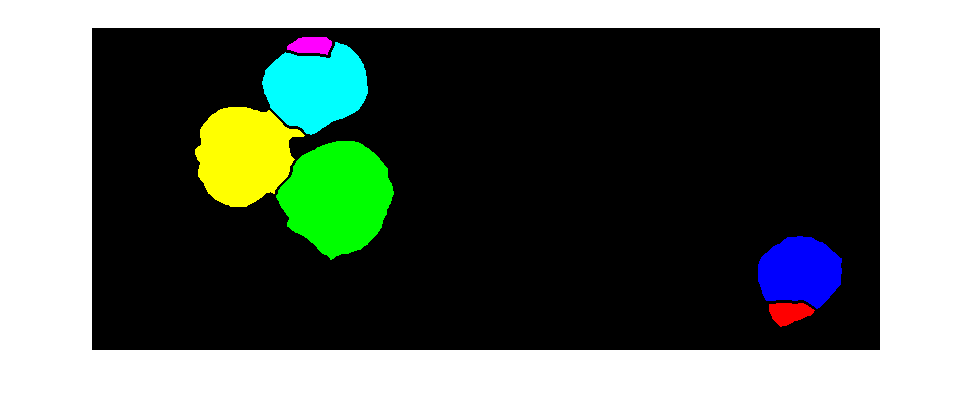
\includegraphics[width=\textwidth]{img/celluleConCito.png}
        \caption{ }
        \label{fig:alltheregions}
    \end{subfigure}
    \begin{subfigure}[b]{0.6\textwidth}
		
\includegraphics[width=\textwidth]{img/conteggioNuclei(noWatersheed).png}
		\caption{ }
		\label{fig:onlybigregions}
	\end{subfigure}
	\caption{(a) All the regions, (b) Only big regions}
	\label{fig:counting}
\end{figure}

\bigskip

This result is not really good in order to have a good segmentation. But it gives us the idea to implement a region-merging function. 
\subsection{Region-Merging}
In order to obtain a merge of the areas we have followed this approach. As first step we separate in two different images the small areas and the big areas, because we want to know about every small area to which of the big areas it belongs. The threshold used to create these tow different images is the medium of the biggest region that there is in the image. To know it we use the minimum distance between the centroids of one small area and all centroids of  the big areas. Then as soon as we labelled every area and we calculated all the centroids we can know what are the areas with minimum distance using the Euclidean distance formula. Now is possible to isolate the two areas \ref{fig:areas}. To merge them we use the function $imclose$ with a disk element with 5 of radius \ref{fig:mergeareas}. Now we can join this result with the image with over-segmentations using the mathematics union operator \ref{fig:unionimage}.
\begin{figure}
	\begin{center}
		\centering
		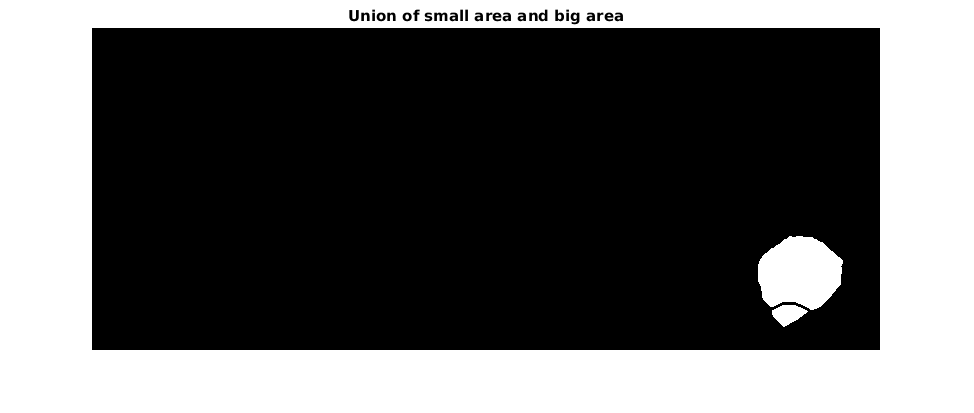
\includegraphics[scale=0.5]{img/final/unionareas.png}
		\caption{Union of two different areas}
		\label{fig:areas}
	\end{center}
\end{figure}
\begin{figure}
	\begin{center}
		\centering
		
\includegraphics[scale=0.5]{img/final/areamerging.png}
		\caption{Merge of two areas}
		\label{fig:mergeareas}
	\end{center}
\end{figure}
\begin{figure}
	\begin{center}
		\centering
		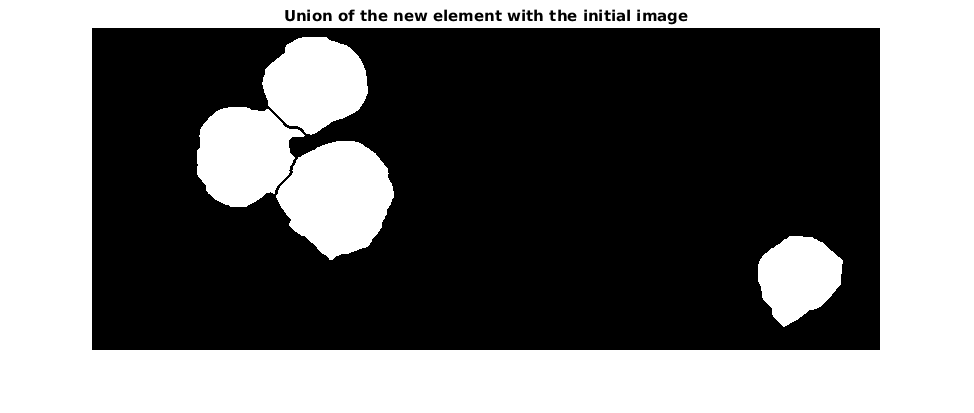
\includegraphics[scale=0.5]{img/final/finalresult.png}
		\caption{Union of initial image and new area}
		\label{fig:unionimage}
	\end{center}
\end{figure}
